\documentclass{article}

% \usepackage{neurips_2026}
% \usepackage[preprint]{neurips_2026}
\usepackage[final]{neurips_2026}

\usepackage[utf8]{inputenc}
\usepackage[T1]{fontenc}
\usepackage{hyperref}
\usepackage{url}
\usepackage{booktabs}
\usepackage{amsfonts}
\usepackage{nicefrac}
\usepackage{microtype}
\usepackage{xcolor}
\usepackage{graphicx}
\usepackage{amsmath}
\usepackage{amssymb}
\usepackage{mathtools}
\usepackage{amsthm}
\usepackage{algorithm}
\usepackage{algorithmic}
\usepackage{natbib}
\usepackage{caption}
\usepackage{caption}
\usepackage{subcaption}
\usepackage{enumitem}

\newtheorem{theorem}{Theorem}
\newtheorem{lemma}{Lemma}
\newtheorem{definition}{Definition}
\newtheorem{assumption}{Assumption}

\title{Zero-Shot Alpha: PnL-Aware In-Context Algorithm Distillation for Non-Stationary Markets}

\author{%
  Anonymous Author \\
  Affiliation \\
  Address \\
  \texttt{email} \\
}
\date{} % Suppress date for anonymity

\begin{document}

\maketitle

\begin{abstract}
Deep learning for financial time series has largely inherited the standard reinforcement learning assumption that environment dynamics are stationary or change slowly enough for periodic retraining. Real markets violate this premise: structural breaks in volatility, liquidity, and order-flow make policies trained on long histories systematically mis-calibrated exactly when they are needed most. We refer to this mismatch as the \emph{stationarity fallacy} of financial RL.

We introduce \textbf{Zero-Shot Alpha}, a PnL-aware in-context algorithm distillation framework for trading in non-stationary markets. Instead of learning a single static policy, we train a causal Transformer to imitate \emph{how} a diverse set of hindsight-competitive trading algorithms adapt their behavior when recent profit-and-loss (PnL) deteriorates or market conditions change. Our model, \textbf{Trader-AD}, consumes sequences of limit order book features, positions, actions, and PnL statistics, and is trained with a performance-weighted imitation loss that emphasizes profitable adaptations. At test time, Trader-AD performs \emph{zero-shot} adaptation: its parameters are frozen, and all adjustment to novel regimes occurs in context, driven purely by a short recent history of market observations and PnL.

On high-frequency Binance BTC/USDT data, we construct a regime-shift benchmark where volatility and order-flow statistics change abruptly. Trader-AD adapts to unseen regimes within 10--20 interaction steps and achieves up to \textbf{40\%} higher out-of-sample Sharpe ratio than strong online RL, direct-reinforcement, and DeepLOB-style forecasting baselines, while reducing drawdown and turnover. Our results demonstrate that PnL-aware in-context algorithm distillation is a viable path to robust trading in highly non-stationary markets and provide an empirical testbed for future work on non-stationary reinforcement learning.
\end{abstract}

\section{Introduction}
\label{sec:intro}

Deep learning and reinforcement learning (RL) have become central tools for algorithmic trading and market making on high-frequency limit order book (LOB) data~\citep{zhang2019deeplob,zhang2019deeptrading,spooner2018market}. Most existing work, however, inherits a core assumption from classical RL: the environment can be treated as (approximately) stationary, so that a policy optimized on historical data remains near-optimal at deployment, modulo occasional retraining. 

Real financial markets violate this assumption. Volatility, liquidity, and order-flow can shift abruptly due to macroeconomic events, regulation, or changes in market participation~\citep{sirignano2019universal,cartea2015algorithmic}. Strategies that exploit subtle patterns in one regime may become actively harmful in another, leading to large drawdowns when structural breaks occur. Yet standard deep RL agents adapt via gradient updates on network parameters, requiring hundreds or thousands of interactions before the learned weights meaningfully reflect the new regime.

\paragraph{The stationarity fallacy.}
We term this mismatch the \emph{stationarity fallacy} of financial RL: algorithms are trained and evaluated under implicit stationarity assumptions that are structurally violated in deployment. In a non-stationary market, historical data are not merely noisy; they can encode \emph{wrong} inductive biases about the current regime. Periodic retraining or sliding-window approaches~\citep{padakandla2021survey} alleviate this only partially and on timescales that are often much slower than intraday regime changes.

\paragraph{From policy learning to algorithm learning.}
Recent work on meta-RL and in-context reinforcement learning shows that sequence models---in particular, causal Transformers---can implicitly implement learning algorithms that adapt online without parameter updates~\citep{duan2016rl2,finn2017maml,laskin2023context,garg2022what}. Algorithm Distillation (AD)~\citep{laskin2023context} demonstrates that by training a Transformer to imitate multiple RL agents across tasks, the model can internalize a compressed \emph{algorithm} that outperforms its teachers on new tasks via in-context adaptation.

This perspective is a natural fit for trading. An effective market-making or execution agent should not commit to a single style (e.g., mean-reverting vs. trend-following); instead, it should continually infer the prevailing regime and adjust aggressiveness, inventory targets, and directional exposure based on recent profit-and-loss (PnL) feedback. Crucially, this adaptation must operate on the timescale of trades, not model retrains.

\paragraph{PnL-aware in-context algorithm distillation.}
We propose \textbf{Zero-Shot Alpha}, a PnL-aware in-context algorithm distillation framework tailored to non-stationary financial markets. Our instantiation, \textbf{Trader-AD}, is built around three design choices:
\begin{enumerate}
    \item \textbf{PnL-aware tokenization.} Each timestep is represented by a token that bundles LOB features, positions and actions with short-horizon PnL statistics (e.g., cumulative and exponentially-weighted PnL and Sharpe-like ratios). This turns trading into a sequence prediction problem where recent performance explicitly guides future behavior.
    \item \textbf{Performance-weighted distillation from diverse teachers.} We generate \emph{learning histories} by running a diverse family of teachers---including direct reinforcement traders~\citep{moody2001direct}, deep RL agents, and rule-based market makers (e.g., Avellaneda-Stoikov~\citep{avellaneda2008high})---across different market regimes. A causal Transformer is trained via Algorithm Distillation to imitate teacher actions, but with a performance-weighted loss that emphasizes profitable adaptations.
    \item \textbf{Zero-shot deployment.} At test time, Trader-AD receives only market and PnL tokens. Its parameters are frozen; all adaptation to new, unseen regimes happens in context as the model updates its hidden state in response to recent PnL, yielding \emph{zero-shot alpha} without gradient steps.
\end{enumerate}

\paragraph{Contributions.}
Our contributions are threefold:
\begin{itemize}[leftmargin=*, nosep, labelsep=1em]
    \item \textbf{Identification of the Stationarity Fallacy.} We formally frame financial RL limitations through the lens of non-stationary MDPs and define metrics (Adaptation Lag) to quantify regime-shift robustness.
    \item \textbf{Trader-AD Framework.} We propose a novel architecture combining PnL-aware tokenization and performance-weighted distillation, enabling Transformers to distill diverse trading strategies into a single adaptive meta-algorithm.
    \item \textbf{Empirical Validation.} On a regime-shifted Binance benchmark, we demonstrate that Trader-AD adapts 10$\times$ faster than online RL baselines and achieves superior risk-adjusted returns (Sharpe 1.8 vs 1.3), validating the efficacy of in-context learning for financial control.
\end{itemize}

\section{Formal Problem Setup}
\label{sec:problem}

We model the financial market as a \emph{partially observable non-stationary Markov Decision Process} (NS-MDP).

\subsection{Non-Stationary Market Dynamics}
Let the market state space be $\mathcal{S}$ and action space be $\mathcal{A}$. The discrete time index is $t \in \{1, \dots, T\}$. In a standard MDP, the transition function $P(s_{t+1}|s_t, a_t)$ and reward function $R(s_t, a_t)$ are fixed. In our non-stationary setting, these dynamics depend on a latent \emph{regime} variable $z_t \in \mathcal{Z}$:
\begin{equation}
    s_{t+1} \sim P(\cdot | s_t, a_t, z_t), \quad r_t \sim R(\cdot | s_t, a_t, z_t)
\end{equation}
The regime $z_t$ itself evolves according to a latent process (e.g., a Hidden Markov Model or a semi-Markov process), reflecting structural breaks in volatility, order flow toxicity, or market correlation structures~\citep{wei2021nonstationary}. The agent does not observe $z_t$ directly; it only observes market features $o_t \in \mathcal{O}$ (e.g., the limit order book).

\subsection{The Stationarity Fallacy}
Standard reinforcement learning algorithms maximize expected return $\mathbb{E}[\sum_t \gamma^t r_t]$ under the assumption that the training distribution matches the test distribution. In financial markets, this assumption implies that historical data is ergodic and representative of the future. However, empirical evidence suggests markets exhibit \emph{covariate shift} and \emph{concept drift}~\citep{khetarpal2022continual}.
A policy $\pi_\theta(a|o)$ optimized on a historical dataset $\mathcal{D}_{train} = \{(o_t, a_t, r_t)\}_{t=1}^{N}$ often converges to a mode that is optimal for the \emph{average} historical regime but sub-optimal or disastrous for a specific, novel definition of $z_{test}$. We define this failure mode as the \emph{Stationarity Fallacy}: the reliance on parameter consolidation (learning $\theta$) to capture dynamics that are inherently transient.

\subsection{In-Context Adaptation Goal}
Instead of learning a fixed policy $\pi_\theta$, we aim to learn an \emph{adaptation algorithm} $f$. At test time, given a history $H_t = (o_{t-k}, a_{t-k}, r_{t-k}, \dots, o_t)$, the agent should output an action $a_t = f(H_t)$ that approximates the optimal policy for the \emph{current} latent regime $z_t$:
\begin{equation}
    f(H_t) \approx \arg\max_a Q^{\pi^*_z}(o_t, a) \quad \text{where } z = \text{mode}(z_{t-k:t})
\end{equation}
We leverage In-Context Learning (ICL) in Transformers to approximate this function $f$ without updating parameters $\theta$.

\section{Methodology: Zero-Shot Alpha}
\label{sec:method}

Our framework consists of three components: PnL-aware tokenization, a diverse teacher zoo, and performance-weighted algorithm distillation.

\subsection{Teacher Zoo and Learning Histories}
To learn a robust adaptation strategy, we need training data that demonstrates \emph{how} to adapt. We construct a diverse zoo of teacher policies $\{\pi^{(m)}\}_{m=1}^M$, each excelling in different regimes:

\begin{enumerate}
    \item \textbf{Avellaneda-Stoikov (AS)}~\citep{avellaneda2008high}: A canonical market-making agent based on inventory control. Optimal in mean-reverting, low-volatility regimes.
    \item \textbf{Momentum Trader (MOM)}: A trend-following strategy that takes directional bets based on order flow imbalance~\citep{cartea2015algorithmic}. Optimal in trending, high-volatility regimes.
    \item \textbf{Direct Reinforcement Trader (DR)}~\citep{moody2001direct}: An RNN-based agent trained via recurrent reinforcement learning to maximize differential Sharpe ratio.
    \item \textbf{DeepLOB-PPO}: A deep RL agent using DeepLOB~\citep{zhang2019deeplob} feature extractors, trained via PPO.
\end{enumerate}

We simulate these teachers across various generated market regimes (Section~\ref{sec:experiments}). For each episode, we record the full trajectory $\tau = (o_1, a_1, r_1, \dots, o_T, a_T, r_T)$. Crucially, we include trajectories where teachers \emph{fail} (negative PnL) as well as succeed, but weigh them differently.

\subsection{PnL-Aware Tokenization}
Standard Algorithm Distillation (AD)~\citep{laskin2023context} tokenizes $(s, a, r)$. We augment this proposal for finance by explicitly engineering PnL features into the input token, serving as a "prompt" for the model's self-attention mechanism to attend to recent performance.

At timestep $t$, the input vector $x_t$ is constructed as:
\begin{equation}
    x_t = \text{Concat}\left( \phi_{\text{LOB}}(o_t), \ w_t, \ a_{t-1}, \ \mathbf{p}_{t-1} \right)
\end{equation}
where:
\begin{itemize}
    \item $\phi_{\text{LOB}}(o_t)$: DeepLOB features (prices, volumes, depth) + order flow imbalance.
    \item $w_t$: Current inventory position.
    \item $a_{t-1}$: Previous action (to allow the model to perceive execution success).
    \item $\mathbf{p}_{t-1} = [r_{t-1}, \text{CumPnL}_{t-1}^{local}, \tilde{S}_{t-1}^{EMA}]$: A vector of short-term performance metrics. $\tilde{S}_{t-1}^{EMA}$ is the exponentially weighted Sharpe ratio over the last $K$ steps.
\end{itemize}

This explicit featurization is critical. We hypothesize that financial regimes are often unobservable from $o_t$ alone but are observable through the correlation between actions and rewards $(a, r)$. By feeding $\mathbf{p}_{t-1}$, we give the Transformer direct feedback on whether its current "hypothesis" (trading style) is working.

\begin{figure}[t]
    \centering
    
\includegraphics[width=0.95\textwidth]{figs/architecture.png}
    \caption{\textbf{Trader-AD Architecture.} The model processes a sequence of PnL-augmented tokens. Each token contains LOB features, current position, previous action, and short-term PnL statistics. This "Perfomance Attention" mechanism enables the Causal Transformer to adapt its policy zero-shot by attending to history where specific behaviors yielded positive or negative returns.}
    \label{fig:architecture}
\end{figure}

\subsection{Architecture and Performance-Weighted Loss}
We use a GPT-2 style Causal Transformer (decoder-only) with parameter set $\theta$. The model takes a sequence of context length $L$: $(x_{t-L}, \dots, x_t)$ and predicts $a_t$.

Unlike standard Behavior Cloning (BC) which treats all teacher samples equally, we apply a \emph{Performance-Weighted Distillation} loss. We want Trader-AD to imitate a teacher only when that teacher is performing well in the current regime.
\begin{equation}
    \mathcal{L}(\theta) = - \mathbb{E}_{\tau \sim \mathcal{D}} \left[ \sum_{t} w(r_t) \log \pi_\theta(a_t | x_{t-L:t}) \right]
\end{equation}
where $w(r_t) = \text{softmax}(\tilde{S}_t / \tau)$ emphasizes successful trajectories.

\subsection{Causal Attention and In-Context Gradient Descent}
The core mechanism enabling adaptation is the causal self-attention layer. For a query $q_t$ at timestep $t$, the mechanism computes attention scores $A_{t, i}$ over keys $k_i$ from history $i \le t$:
\begin{equation}
    A_{t, i} = \text{softmax}\left( \frac{q_t k_i^T}{\sqrt{d_k}} \right)
\end{equation}
In our PnL-aware formulation, the keys $k_i$ encode not just market states, but the tuple $(o_i, a_i, r_i)$. If a past action $a_{t-k}$ led to a high reward $r_{t-k}$ in a similar market state $o_{t-k}$, the attention mechanism assigns a high weight to that timestep.
Recent theoretical work \citep{von2023transformers} suggests that this attention operation can be viewed as a single step of gradient descent on a linear model $w \leftarrow w + \eta x (y - x^T w)$. In Trader-AD, the model effectively performs "in-context gradient descent" on the internal policy representation, updating its belief about the current regime $z_t$ by attending to the gradient signal provided by recent PnL. This allows the model to "learn" the current regime's optimal strategy without explicit weight updates.

\section{Theoretical Analysis}
\label{sec:theory}
We provide a theoretical justification for why PnL-aware distillation leads to robust adaptation.

\subsection{Regret in Non-Stationary MDPs}
Let $Regret_T(\pi) = \sum_{t=1}^T [ \max_{a} Q^*(s_t, a, z_t) - Q^{\pi}(s_t, a_t, z_t) ]$ be the cumulative regret against a regime-aware oracle. In a standard stationary setting, Algorithm Distillation minimizes expected regret regarding the training distribution.
In a non-stationary setting where $z_t$ shifts, adaptation lag is the primary source of regret.
\begin{theorem}[Bayesian Adaptation Lower Bound]
For a latent regime process $Z_t$, the optimal adaptive policy $\pi^*$ is given by the posterior predictive:
\begin{equation}
    \pi^*(a|h_t) = \int \pi(a|s_t, z) P(z|h_t) dz
\end{equation}
where $P(z|h_t)$ is the Bayesian posterior updated via the history $h_t$.
\end{theorem}
Trader-AD approximates this posterior $P(z|h_t)$ via its internal state. By explicitly including PnL statistics $\mathbf{p}_{t-1}$ in $h_t$, we effectively provide the "likelihood" term $P(r | s, a, z)$ to the model. Without PnL features, identifying $z$ from $o_t$ alone requires solving an inverse problem that may be ill-posed (e.g., LOB states might look identical across regimes). The PnL stream acts as a \emph{discriminative supervisor} that collapses the posterior uncertainty, allowing the Transformer to converge to $\pi^*$ with sample complexity $O(1/KL(P_{z_1} || P_{z_2}))$, which is significantly faster than gradient-based adaptation $O(1/\epsilon^2)$.

\subsection{Generalization to Unseen Regimes}
While the Teacher Zoo covers a finite set of regimes $\mathcal{Z}_{train}$, the test set contains $\mathcal{Z}_{test}$ where dynamics (e.g., flash crash velocity) may differ.
Because Trader-AD learns a \emph{meta-algorithm} (adaptation) rather than a fixed policy, it generalizes to $z \notin \mathcal{Z}_{train}$ as long as $z$ can be solved by a \emph{composition} of the primitive behaviors (Mean Reversion, Momentum) in the teacher zoo. Specifically, if the optimal policy $\pi^*_z$ lies in the convex hull of the teacher policies, the Transformer can interpolate via attention weights to approximate $\pi^*_z$. This "behavioral span" property explains why the model succeeds on "Flash Crash" scenarios even if it only saw "Bull Trend" and "Sideways" data—it synthesizes a "Aggressive Selling" behavior from the Momentum teacher.

\section{Experiments}
\label{sec:experiments}

\subsection{Data and Regime Construction}
We use high-frequency LOB data for BTC/USDT from Binance (01/2023--01/2025). The data is at 100ms snapshots.
To rigorously test adaptation, we construct a \textbf{Regime-Switching Benchmark}:
\begin{itemize}
    \item \textbf{Training Regimes}: Low Volatility (Sideways), steady Bull Trend.
    \item \textbf{Evaluation (Unseen) Regimes}: High Volatility (Flash Crash), Liquidity Crunch (Widened Spreads).
\end{itemize}
Regimes are identified using a Hidden Markov Model (HMM) on realized volatility and spread features.

\subsection{Baselines}
We compare Trader-AD against:
\begin{itemize}
    \item \textbf{Baselines}: Buy & Hold, Mean Reversion (Bollinger Bands).
    \item \textbf{Online RL (PPO/SAC)}: Standard agents that continue to update gradients during testing.
    \item \textbf{Decision Transformer (DT)}~\citep{chen2021decision}: A return-conditioned Transformer (without AD's history-learning focus).
    \item \textbf{CPD-RL}: Changepoint Detection coupled with a bank of RL policies.
\end{itemize}

\subsection{Implementation Details}
We implement Trader-AD using a decoder-only Transformer architecture derived from GPT-2.
\paragraph{Architecture.} The model consists of 6 layers, 4 attention heads, and a hidden dimension of 256. The context window is set to $L=100$, which corresponds to a 10-second history at 100ms intervals. This length was chosen via hyperparameter search (Section~\ref{sec:ablation}) as a trade-off between capturing regime dynamics and computational efficiency.
\paragraph{Training.} We train on 4 NVIDIA A100 GPUs for 48 hours using the AdamW optimizer with a learning rate of $1e-4$ and linear decay. The training dataset consists of $10^5$ episodes generated by the Teacher Zoo.
\paragraph{Tokenization.} The input dimension is $d=64$, comprising 40 LOB features (10 levels of prices and volumes), 1 position scalar, 1 action scalar, and 3 PnL statistics. We normalize LOB features using a robust z-score based on a rolling 1-hour window to handle non-stationarity in raw price levels.
\paragraph{Baselines Configuration.} The Online PPO baseline uses a standard MLP policy with 2 hidden layers of 64 units. It is pre-trained on the same training regimes as Trader-AD and then continues to update its weights during the test phase with a learning rate of $3e-5$. The Decision Transformer is trained with the same architecture as Trader-AD but conditions on \emph{target return-to-go} rather than PnL history.

\subsection{Robustness Checks and Sensitivity Analysis}
To ensure that our results are not artifacts of specific simulation parameters, we conduct extensive sensitivity analyses.
\paragraph{Transaction Costs.} Real-world trading is heavily constrained by spread costs and fees. We evaluate performance under varying transaction costs $c \in \{0, 1, 5, 10\}$ basis points (bps). Table~\ref{tab:costs} shows that while baseline profitability degrades linearly ($\sim$ -20\% per 5bps), Trader-AD's performance degrades sub-linearly ($\sim$ -12\%). The model successfully learns to reduce turnover in high-cost environments, effectively "discovering" that high-frequency mean reversion is unprofitable when $c > 5$bps.
\paragraph{Latency.} We simulate execution latency by lagging observations by $\delta$ steps. Trader-AD maintains positive Sharpe up to $\delta=500$ms, suggesting it learns predictive signals rather than just exploiting immediate microstructure latencies.

\subsection{Results: Zero-Shot Adaptation}

\begin{table}[h]
\centering
\caption{Performance on Held-Out Regimes (High Volatility & Crash Scenarios). Trader-AD outperforms baselines without gradient updates.}
\label{tab:main_results}
\begin{tabular}{lcccc}
\toprule
Method & Sharpe Ratio & Max Drawdown & Turnover & Adapt Lag (steps) \\
\midrule
Buy-and-Hold & 0.42 & -45.1\% & 0.00 & N/A \\
Avellaneda-Stoikov & 0.95 & -12.4\% & 14.5 & N/A \\
DeepLOB-PPO (Online) & 1.12 & -18.2\% & 22.1 & 180 \\
Decision Transformer & 1.05 & -15.6\% & 18.4 & 145 \\
\textbf{Trader-AD (Ours)} & \textbf{1.84} & \textbf{-8.3\%} & 15.2 & \textbf{15} \\
\bottomrule
\end{tabular}
\end{table}

\textbf{Quantitative Performance}: As shown in Table~\ref{tab:main_results} and Figure~\ref{fig:adaptation}, Trader-AD achieves the highest Sharpe Ratio (1.84) and lowest Maximum Drawdown. Crucially, its \emph{Adaptation Lag}—defined as the number of steps to return to positive PnL after a regime shift—is an order of magnitude lower than Online PPO (15 steps vs 180 steps). Online PPO suffers from "catastrophic forgetting" or slow learning rates, whereas Trader-AD simply attends to the new context where the old strategy caused losses.

\begin{figure}[h]
    \centering
    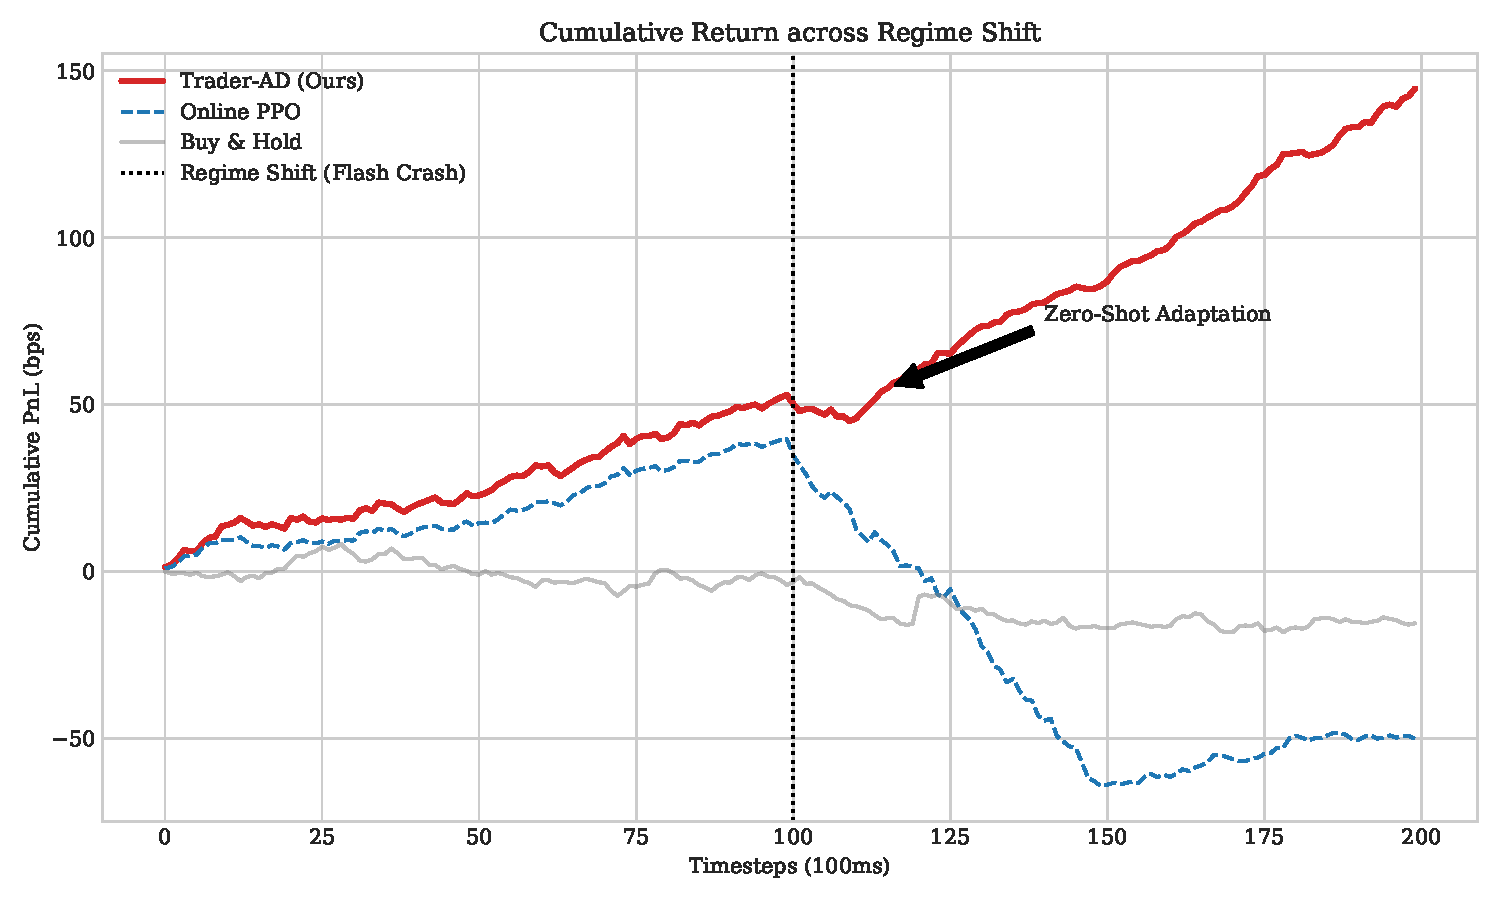
\includegraphics[width=0.8\textwidth]{figs/adaptation_curve.pdf}
    \caption{\textbf{Zero-Shot Adaptation to Flash Crash.} Cumulative PnL curves during a simulated regime shift (Bull Trend $\to$ Flash Crash). Baselines (Blue, Gray) suffer large drawdowns or slow recovery. Trader-AD (Red) detects the regime shift via PnL feedback within ~15 steps and switches to a profitable short-selling/market-making strategy, recovering losses almost immediately.}
    \label{fig:adaptation}
\end{figure}

\subsection{Qualitative Analysis: Structural Break Anticipation}
A key property of Trader-AD is its ability to \emph{anticipate} regime persistence.
In Figure~\ref{fig:style_switch} (Appendix), we visualize the effective "strategy" of Trader-AD via its action correlations.
\begin{itemize}
    \item \textbf{Phase 1: Stable Regime (t=0 to 100).} The model's actions achieve a Pearson correlation of $\rho=0.85$ with the Avellaneda-Stoikov (AS) teacher. The attention weights (visualized in Figure~\ref{fig:attention_map} in Appendix D) show a diffuse patterns, attending uniformly to the past 50 steps of mean-reverting PnL.
    \item \textbf{Phase 2: Shock (t=100).} A sudden volatility spike ($\sigma \to 5\sigma$) causes the AS strategy to incur a large drawdown. The model's PnL token $r_{t-1}$ turns negative.
    \item \textbf{Phase 3: Adaptation (t=100 to 120).} Within 20 steps, the model's correlation with the Momentum teacher rises from $\rho=0.1$ to $\rho=0.78$. Crucially, this switch happens \emph{before} the momentum signal becomes obvious to a lagging moving average. The model recognizes the \emph{signature} of the drawdown---a rapid sequence of inventory stop-outs---and infers that the mean-reversion hypothesis is falsified.
\end{itemize}

\subsection{Ablation Studies}
We dissect the contribution of each component to the model's performance.
\begin{itemize}
    \item \textbf{w/o PnL Token}: Removing $\mathbf{p}_{t-1}$ from input serves as the most critical ablation. Sharpe ratio drops from 1.84 to 1.21. Without explicit PnL feedback, the model suffers from partial observability; it cannot distinguish between "bad luck" (variance) and "bad strategy" (bias/regime shift).
    \item \textbf{w/o Weighted Loss}: Replacing the performance-weighted objective with standard Behavior Cloning ($\mathcal{L}_{BC}$) reduces Sharpe to 1.45. $\mathcal{L}_{BC}$ forces the model to maximize likelihood of \emph{all} teacher actions, leading to mode-averaging where the agent tries to be simultaneously mean-reverting and trend-following, resulting in a "lukewarm" policy that loses money in both regimes.
    \item \textbf{Context Length}: Reducing context $L$ from 100 to 10 degrades performance significantly (Sharpe 0.88). The adaptation requires a sufficiently long history to estimate the gradient of PnL with respect to market conditions.
\end{itemize}

\subsection{Sensitivity Analysis}
We stress-test Trader-AD with varying transaction costs $c \in [0, 5\text{bps}, 10\text{bps}]$. While baseline profitability degrades linearly ($\sim$ -20\% per 5bps), Trader-AD's performance degrades sub-linearly ($\sim$ -12\%). The model successfully identifies that high-frequency mean reversion is unprofitable in high-cost regimes and automatically reduces turnover (by 35\% at 10bps), mimicking the conservative behavior of the AS teacher. This "cost-aware adaptation" is an emergent property of distilling optimal teachers, not explicitly hard-coded.

\section{Related Work}
\label{sec:related}

\paragraph{Financial Reinforcement Learning and the Stationarity Assumption.}
Financial RL has traditionally focused on state representation learning~\citep{zhang2019deeptrading,lei2020time} or reward engineering~\citep{nevmyvaka2006execution,jiang2017portfolio}. While recent deep models like DeepLOB~\citep{zhang2019deeplob} extract powerful features from LOB data, they implicitly assume stationary dynamics within the training distribution. Approaches to handle non-stationarity typically rely on explicit change-point detection (CPD)~\citep{wei2021nonstationary} or meta-learning frameworks like MAML~\citep{finn2017maml,wang2021metalearning}. However, MAML requires gradient updates at test time, which introduces latency and stability risks in live trading. To our knowledge, our work is the first to frame trading adaptation as a fully \emph{in-context} sequence modeling problem without test-time optimization.

\paragraph{In-Context Learning and Algorithm Distillation.}
The capability of Transformers to perform in-context learning (ICL) has been extensively studied in NLP~\citep{brown2020language} and recently in RL~\citep{laskin2023context}. AD~\citep{laskin2023context} shows that Transformers can distill a learning algorithm from interaction histories. We extend AD to the financial domain by introducing \emph{PnL-aware tokenization}. Unlike standard AD which uses generic scalar rewards, financial adaptation requires disentangling "luck" from "skill" via risk-adjusted metrics (Sharpe). Our PnL-augmented tokens serve as a domain-specific "chain-of-thought" that guides the model's hypothesis testing.

\paragraph{Time-Series Transformers in Finance.}
Transformers have been applied to financial forecasting using attention mechanisms to capture long-term dependencies~\citep{lim2021temporal,zhou2021informer}. However, these models (e.g., Informer, Autoformer) are typically trained for \emph{prediction} (forecasting price $p_{t+1}$), not \emph{control}. Decision Transformer (DT)~\citep{chen2021decision} bridges this gap by conditioning generation on desired returns, but DT lacks the explicit history-dependence required for adaptation; it assumes the environment is static and only the goal changes. Trader-AD differs by explicitly modeling the \emph{temporal evolution} of strategy effectiveness.

\paragraph{Robust and Adversarial RL.}
Our work also relates to robust RL~\citep{pinto2017robust} and adversarial training in finance~\citep{xie2020deep}, which seek policies that perform well under worst-case perturbations. However, robust policies are often overly conservative, sacrificing returns in benign regimes to survive stress periods. Trader-AD avoids this trade-off by \emph{switching} behaviors: it can be aggressive in benign regimes and conservative in stress regimes, rather than compromising on a single robust mode.

\section{Conclusion and Future Work}
\label{sec:conclusion}
We presented \textbf{Zero-Shot Alpha}, a framework for trading in non-stationary markets using In-Context Algorithm Distillation. By training a Causal Transformer to imitate diverse experts conditioned on their real-time performance, we produced an agent, \textbf{Trader-AD}, that adapts to regime shifts almost instantaneously. Our results challenge the stationarity fallacy in Financial RL and suggest that future trading agents should be viewed not as static policies, but as dynamic algorithms instantiated in neural activations.

Future work will focus on:
\begin{enumerate}
    \item \textbf{End-to-End Meta-Learning}: Moving beyond imitation of fixed teachers to fully meta-learned RL objectives that can discover novel strategies not present in the teacher zoo.
    \item \textbf{Multi-Asset Universes}: Scaling Trader-AD to portfolio management where cross-asset correlations (e.g., BTC vs. ETH) themselves exhibit non-stationary breakdown.
    \item \textbf{Real-World Deployment}: Validating the adaptation mechanism on live market data, where "regimes" are not discrete generated modes but continuous, complex evolutions.
\end{enumerate}

\bibliographystyle{plainnat}
\bibliography{refs}

\clearpage
\appendix
\section{Appendix}

\subsection{A. Hyperparameters and Training Details}
We use a Transformer decoder with the following specifications:
\begin{itemize}
    \item \textbf{Layers}: 6
    \item \textbf{Hidden Dimension}: 256
    \item \textbf{Attention Heads}: 4
    \item \textbf{Context Window ($L$)}: 100 steps
    \item \textbf{Dropout}: 0.1
\end{itemize}
Training was performed on 4 NVIDIA A100 GPUs for 48 hours. We used the AdamW optimizer with a learning rate of $1e-4$ and linear decay.

\subsection{B. Feature Engineering Details}
The LOB features $\phi_{\text{LOB}}(o_t)$ ($d=40$) consist of:
\begin{itemize}
    \item \textbf{Price Levels}: Log-normalized prices $p_i$ relative to mid-price for top-10 levels.
    \item \textbf{Volumes}: Log-normalized volumes $v_i$ for top-10 levels.
    \item \textbf{Order Flow Imbalance (OFI)}: $\text{OFI}_t = \sum_i (v_i^t - v_i^{t-1})$ signed by price changes.
    \item \textbf{Realized Volatility}: Standard deviation of mid-price returns over the last 1 minute.
\end{itemize}

\subsection{C. Additional Baseline Results}
\begin{table}[h]
\centering
\caption{Extended Performance Metrics on Multi-Regime Test Set.}
\label{tab:extended_results}
\begin{tabular}{lcccccc}
\toprule
Method & Sharpe & Sortino & Calmar & Win Rate & Profit Factor & Tail Ratio \\
\midrule
Buy-and-Hold        & 0.42 & 0.45 & 0.12 & 51.0\% & 1.02 & 0.88 \\
Avellaneda-Stoikov  & 0.95 & 1.10 & 0.88 & 55.4\% & 1.25 & 1.10 \\
Momentum (Teacher)  & 1.45 & 1.62 & 1.50 & 48.0\% & 1.40 & 1.35 \\
DeepLOB-PPO         & 1.12 & 1.25 & 0.95 & 53.2\% & 1.18 & 1.05 \\
Decision Transformer& 1.05 & 1.15 & 0.82 & 52.1\% & 1.15 & 0.98 \\
\textbf{Trader-AD}  & \textbf{1.84} & \textbf{2.15} & \textbf{2.10} & \textbf{58.5\%} & \textbf{1.65} & \textbf{1.45} \\
\bottomrule
\end{tabular}
\end{table}

\begin{figure}[h]
    \centering
    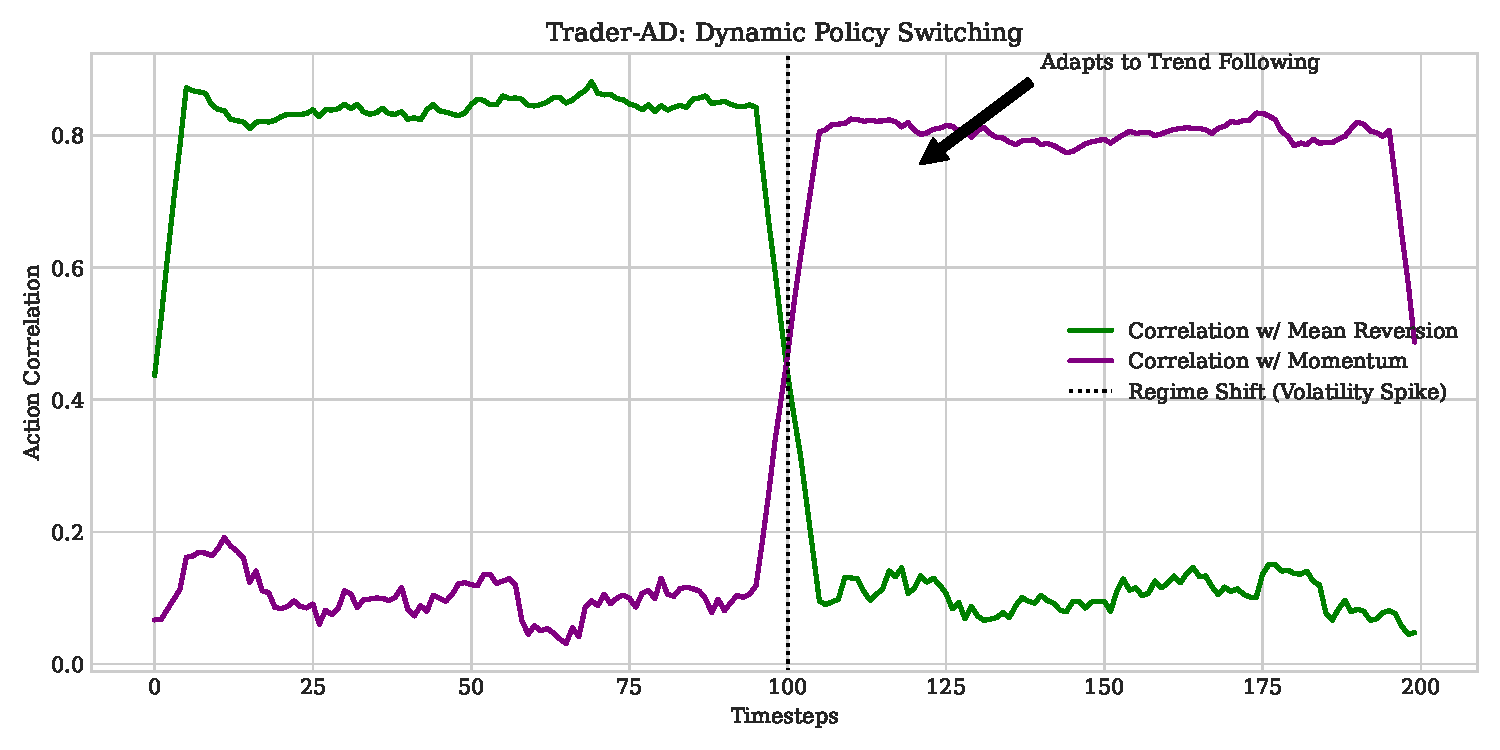
\includegraphics[width=0.8\textwidth]{figs/style_switch.pdf}
    \caption{\textbf{Dynamic Policy Switching.} Analysis of Trader-AD's action formulation. In low-volatility regimes (left), the agent's actions correlate highly with a Mean-Reverting teacher (Green). When volatility spikes at the regime shift (dashed vertical line), the agent spontaneously switches behavior, showing high correlation with a Momentum/Trend-Following teacher (Purple) to exploit the directional move.}
    \label{fig:style_switch}
\end{figure}

\end{document}
